% ---------------------------------------------------------------------------
% Chapter based on a manuscript IN PREPARATION, with a structured abstract
% and a long supplementary table that breaks across pages (longtable).
% ---------------------------------------------------------------------------
\basedon{%
Firstname Lastname, Author Two, Author Three (2026). \textit{Title of the manuscript.} In preparation.}
\chapter{Full Title of the Third Research Chapter}
\setcounter{figure}{0}
\renewcommand{\thefigure}{\thechapter.\arabic{figure}}

\chapterauthors{%
	Firstname Lastname$^{1,*}$, Author Two$^{2}$, Author Three$^{1}$

	\vspace{0.5em}

	$^{1}$Department, University, City, Country

	\vspace{0.25em}

	$^{2}$Second affiliation

	\vspace{0.5em}

	\small
	$^{*}$Corresponding author: \texttt{email@example.org}
}

\begin{chapterabstract}
\noindent\textbf{Background.}
[Text.]

\noindent\textbf{Objective.}
[Text.]

\noindent\textbf{Methods.}
[Text.]

\noindent\textbf{Results.}
[Text.]

\noindent\textbf{Conclusions.}
[Text.]
\end{chapterabstract}

\section{Introduction}
[Text \citep{placeholderArticle2024}.]

\section{Methods}
\subsection{Study overview}
[Text. Protocol parameters are listed in Table~\ref{tab:ch4-long}.]

\section{Results}
[Text referring to Figure~\ref{fig:ch4-main}.]

\begin{figure}[htbp]
	\centering
	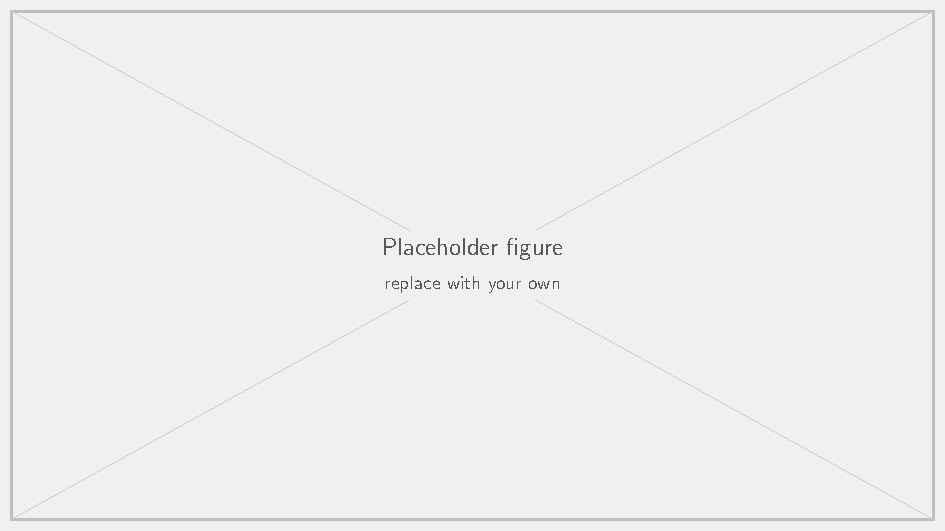
\includegraphics[width=0.8\linewidth]{chapters/chapter3/figures/placeholder.pdf}
	\caption{\textbf{Figure title.} Caption text.}
	\label{fig:ch4-main}
\end{figure}

\section{Discussion}
[Text.]

\section*{Declaration of competing interest}
[Statement.]

\section*{Data availability}
[Statement.]

\section*{Acknowledgements}
[Funding statement.]

% ---------- Supplementary material ----------
\clearpage
\renewcommand{\thefigure}{S\arabic{figure}}
\renewcommand{\thetable}{S\arabic{table}}
\setcounter{figure}{0}
\setcounter{table}{0}
\section{Supplementary}
\subsection{Parameter table}

{\fontsize{8}{10.5}\selectfont
\setlength{\tabcolsep}{3pt}\renewcommand{\arraystretch}{1.25}
\begin{longtable}{@{}>{\raggedright\arraybackslash}p{0.34\linewidth}>{\raggedright\arraybackslash}p{\dimexpr0.66\linewidth-6pt\relax}@{}}
\caption{\textbf{Long table title.} A table that continues across pages.}\label{tab:ch4-long}\\
\toprule
\endfirsthead
\multicolumn{2}{@{}l}{\textit{Table \thetable\ (continued)}}\\
\toprule
\endhead
\bottomrule
\endfoot
\bottomrule
\endlastfoot
	\rowcolor{black!18}\multicolumn{2}{@{}l@{}}{\hspace{3pt}\textbf{Group heading}} \\
	Parameter 1 & Value \\
	Parameter 2 & Value \\
	\rowcolor{black!18}\multicolumn{2}{@{}l@{}}{\hspace{3pt}\textbf{Second group heading}} \\
	Parameter 3 & Value \\
	Parameter 4 & Value \\
\end{longtable}
}

\renewcommand{\thefigure}{\thechapter.\arabic{figure}}

\renewcommand{\thetable}{\thechapter.\arabic{table}}
